\input{../YKY-preamble-PPT.tex}

\usepackage{color}
\usepackage{mathtools}
\usepackage{hyperref}

%\usepackage[backend=biber,style=numeric]{biblatex}
%\bibliography{../AGI-book}
% \renewcommand*{\bibfont}{\footnotesize}

\usepackage{graphicx} % Allows including images
\usepackage{tikz-cd}
\usepackage{tikz}
\usepackage[export]{adjustbox}% http://ctan.org/pkg/adjustbox
\usepackage{verbatim} % for comments
% \usepackage{newtxtext,newtxmath}	% Times New Roman font

% \numberwithin{equation}{subsection}

\newcommand{\underdash}[1]{%
	\tikz[baseline=(toUnderline.base)]{
		\node[inner sep=1pt,outer sep=10pt] (toUnderline) {#1};
		\draw[dashed] ([yshift=-0pt]toUnderline.south west) -- ([yshift=-0pt]toUnderline.south east);
	}%
}%

\DeclareSymbolFont{symbolsC}{U}{txsyc}{m}{n}
\DeclareMathSymbol{\strictif}{\mathrel}{symbolsC}{74}

\newcommand{\highlight}[1]{\colorbox{pink}{$\displaystyle #1$}}

\let\oldtextbf\textbf
\renewcommand{\textbf}[1]{\textcolor{blue}{\oldtextbf{#1}}}

\newcommand{\emp}[1]{{\color{blue}\textbf{#1}}}
\newcommand*\confoundFace{$\vcenter{\hbox{\includegraphics[scale=0.2]{../2020/../confounded-face.jpg}}}$}
\newcommand{\underconst}{\includegraphics[scale=0.5]{../2020/UnderConst.png}}
\newcommand{\witness}{\scalebox{0.6}{$\blacksquare$}}
% \newcommand{\Heytingarrow}{\mathrel{-}\mathrel{\triangleright}}
\providecommand\Heytingarrow{\relbar\joinrel\mathrel{\vcenter{\hbox{\scalebox{0.75}{$\rhd$}}}}}

\begin{document}

\title{\bfseries\color{blue}{\Huge《AGI in 5 minutes》}}
\author{YKY} % Your name
%\institute[] % Your institution as it will appear on the bottom of every slide, may be shorthand to save spacer5t
%{
%Independent researcher, Hong Kong \\ % Your institution for the title page
%\medskip
%\textit{generic.intelligence@gmail.com} % Your email address
%}
\date{\today} % Date, can be changed to a custom date

\maketitle
\pagenumbering{gobble}

\begin{itemize}
	\item 我预计 AGI 会在 5-6 年内出现。
	\item 理由是 因为 BERT/GPT 已经示范了 \\
		 现时计算机的算力 \\
		 已经进入了 AGI 的 ``ballpark'' 范围
	\item BERT/GPT 可以 答问题、写文章、甚至写 code,\\
		这些能力 毫无疑问是 通用智能 的特性
	\item 虽然很多人见到了 BERT/GPT,\\
		但并不意识到它们就是 AGI 的雏型
\end{itemize}

\section*{AGI Early and Current Players}

YKY and Ben Goertzel, founder of OpenCog.  (2009 photo)
\begin{equation}
\vcenter{\hbox{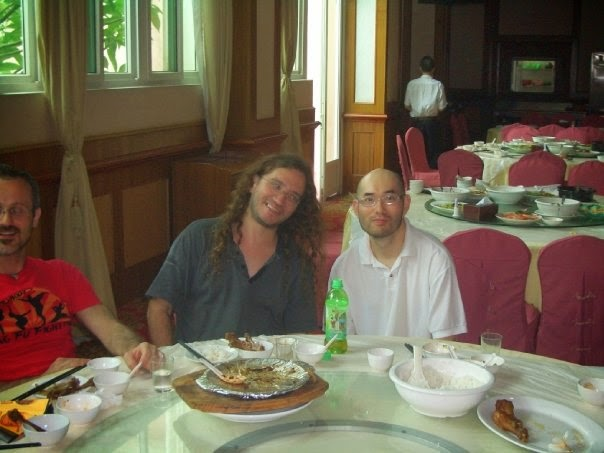
\includegraphics[scale=0.5]{YKY-and-BenGoertzel.jpg}}}
\nonumber
\end{equation}

YKY and Pei Wang(王培), founder of OpenNARS.
\begin{equation}
\vcenter{\hbox{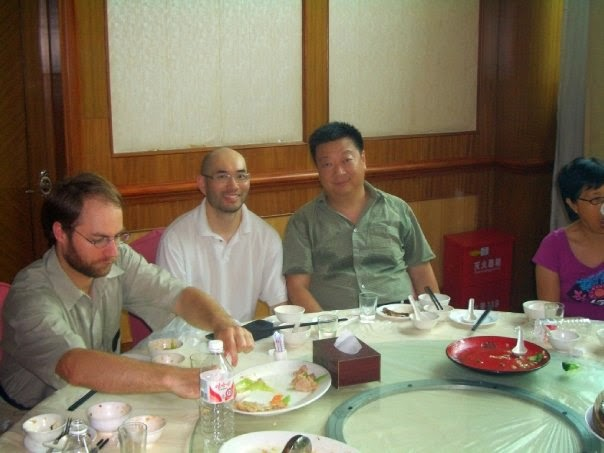
\includegraphics[scale=0.5]{YKY-and-PeiWang.jpg}}}
\nonumber
\end{equation}

\begin{itemize}
	\item OpenCog 和 OpenNARS 都是基于 \textbf{逻辑}的引擎,\\
		但加入了某种 probabilistic 或 uncertainty logic.
	\item 他们的 uncertainty 处理方式有点麻烦,\\
		于是我提出了一种 fuzzy-probabilistic logic (2012 paper) \\
		但没有被采纳,然而这争拗 很可能已不再是重点所在.
	\item 他们是我的前辈也是朋友,也是竞争者,\\
		我非常欣赏他们不遗余力地推广 AGI,\\
		Ben 在全世界 AGI 圈子内很有名,\\
		王培 在国内也培养了很多 AGI 人材,\\
		而 OpenNARS 最近也有国际上的研发者参与
	\item 但我个人觉得 现代 AGI 已被 deep learning 占了主导地位
	\item DeepMind 是现时世界最强的 AGI 研究中心,\\
		他们有些早期成员来自 Ben 的 AGI mailing list.\\
		DeepMind 是一间对 AGI 很著迷的公司,\\
		他们绝对不止于玩玩围棋或 Atari 而已,\\
		正如他们的名称所示。
	\item Ben 早期的项目叫 Novamente,\\
		(他是天才,在南美长大,23岁 PhD) \\
		Novamente 在西班牙语意思是 ``again'',\\
		但也可以理解为 ``new mind''.
\end{itemize}

\section*{Logic as the basis of AGI}

很多人怀疑: 符号逻辑 可以作为 人工智能的基础吗? 

可以看看这本书,作者 Robert Kowalski 就是 Prolog 语言的创始人之一:
\begin{equation}
\vcenter{\hbox{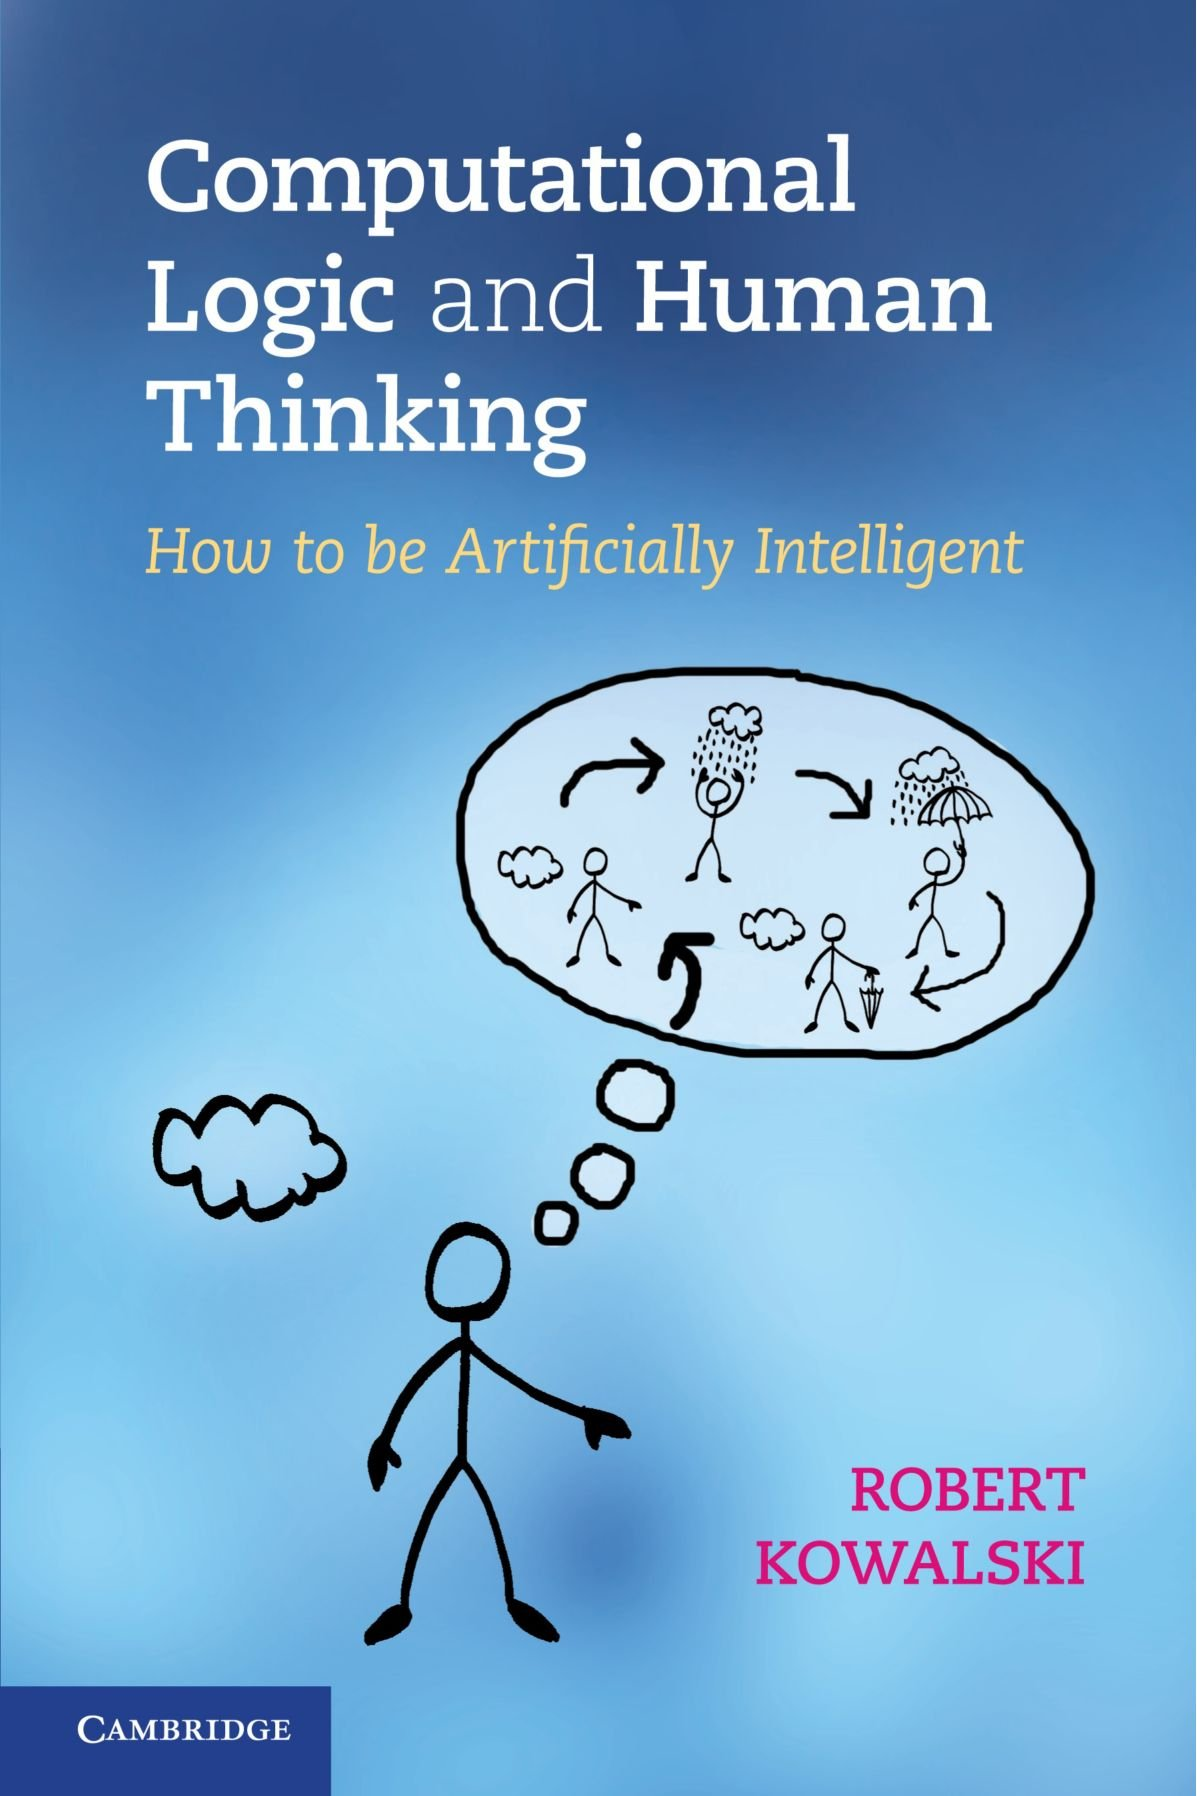
\includegraphics[scale=0.3]{Computational-logic-and-human-thinking_(cover).jpg}}}
\nonumber
\end{equation}

\begin{itemize}
	\item 这本书解释,在逻辑里主要有三种推理模式:\\
		\tab deduction(前向推理)\\
		\tab abduction(溯因推理,找出命题 $A$ 的解释,即 $B \Rightarrow A$) \\
		\tab induction(归纳推理,从事例中总结出,\\
		\tab \tab 例如「所有书呆子都是四眼的」)
	\item 这些逻辑模式,可以涵盖所有人类思维
\end{itemize}

Jerry Hobbs 提出 abductive interpretation of natural language\\
这是用 经典逻辑的方式 解决 \textbf{自然语言理解} 的问题:
\begin{equation}
\vcenter{\hbox{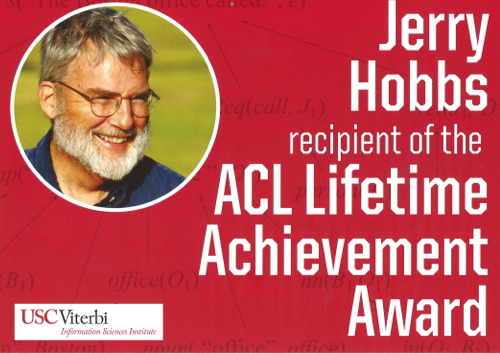
\includegraphics[scale=0.7]{Jerry-Hobbs.png}}}
\nonumber
\end{equation}

\begin{itemize}
	\item 例如:\\
		\tab door-knob 是「门的手把」\\
		\tab school-girl 是「上学的女孩」\\
		\tab machine-gun 是「用机械发子弹的枪」\\
		这些组合词的诠释,各有不同,\\
		它们需要用 abductive reasoning 解释。
\end{itemize}

\section*{The Problem of Logic-Based AI}

\begin{itemize}
	\item 经典逻辑 AI 有个 \textbf{严重问题}: \\
		就是 缺乏 快速/高效率的 \textbf{学习算法},\\
		而学习算法是 AI 的灵魂,\\
		这直接造成了历史上所谓的 ``AI Winter''.
	\item 经典逻辑 AI 要学习 巨量的 逻辑式子,\\
		eg. $\forall x. \; \mbox{Human}(x) \Rightarrow \mbox{Mortal}(X)$ \\
		而这是在一个 discrete lattice 里面搜寻,\\
		换句话说是一种 combinatorial search,\\
		而 search tree 是所有逻辑句子的 syntax,\\
		它的 branching factor 很大,\\
		而在没有 oracle「神喻」的情况下,\\
		就 exactly 像 P $\neq$ NP 那种难解的情况。
	\item 深度学习的 \textbf{革命性}意义,\\
		在于打破了 learning algorithm 的困境.
	\item 注意: 即使现在有了 深度学习,\\
		逻辑 AI 仍然欠缺快速的 learning algorithm,\\
		而这件事没有因为 深度学习的出现而解决。
\end{itemize}

\section*{Hot-swap architecture}

\begin{equation}
\vcenter{\hbox{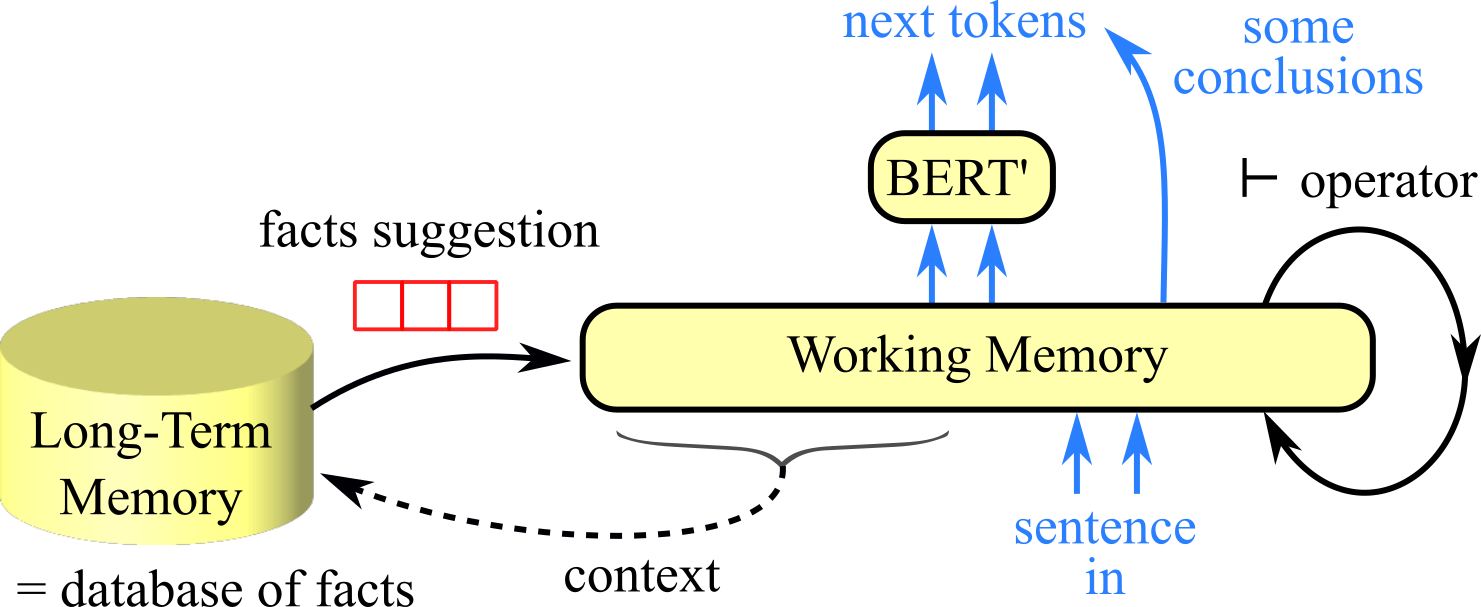
\includegraphics[scale=0.9]{hot-swap-architecture.png}}}
\end{equation}

\begin{itemize}
	\item 问题是 BERT 和 Sym 的 state 是否可以混合?
	\item 主要目的是想将 BERT states 变成 ground states,\\
		则以后可以「接地应用」
	\item 如果可以将 BERT 的知识内容 转移到 Sym,似乎是有益的
	\item 问题是 如果用 RL + Sym 训练 masked language model, \\
		凭什么 觉得 这样 学到的知识 是 grounded?
\end{itemize}

% \section*{References}
% \cc{欢迎提问和讨论}{Questions, comments welcome} \smiley \\ \vspace*{0.4cm}
% \printbibliography

\end{document}
